%Đây là template dùng cho đề cương đề tài tốt nghiệp
%Khoa Công nghệ Thông tin
%Trường Đại học Khoa học Tự nhiên, ĐHQG-HCM

%Liên hệ về mẫu LaTEX này: Thầy Bùi Huy Thông (bhthong@fit.hcmus.edu.vn)
% Bắt đầu nội dung đề cương chi tiết
\begingroup
\addcontentsline{toc}{chapter}{Đề cương chi tiết} \renewcommand{\addcontentsline}[3]{} \renewcommand{\thesection}{\arabic{section}} \renewcommand{\thesubsection}{\thesection.\arabic{subsection}} \renewcommand{\thesubsubsection}{\thesubsection.\arabic{subsubsection}} \renewcommand{\thefigure}{\arabic{figure}} \renewcommand{\thetable}{\arabic{table}}

% Định dạng chapter/section
\titleformat*{\section}{\LARGE\bfseries}
\titleformat*{\subsection}{\Large\bfseries}
\titleformat*{\subsubsection}{\large\bfseries}


\noindent
  \begin{minipage}[c]{0.2\textwidth}
\centering
      
\includegraphics[scale = .35]{logo.png}
  \end{minipage}%
  \begin{minipage}[c]{1.0\textwidth}
\centering \fontsize{10}{16}\selectfont\textbf{TRƯỜNG ĐẠI HỌC KHOA HỌC TỰ NHIÊN\\KHOA CÔNG NGHỆ THÔNG TIN}
  \end{minipage}
\vspace{0.8cm}

  \begin{center}

      %Xác định loại đề tài tốt nghiệp tương ứng: Khóa luận, Thực tập, Đồ án
      \textbf{\large ĐỀ CƯƠNG KHOÁ LUẬN TỐT NGHIỆP} \\
  \end{center}

  %\vspace{.5cm}

  \begin{center}
  %Tên đề tài phải VIẾT HOA

\textbf{\Large PHÁT TRIỂN HỆ THỐNG PHÂN LỚP ẢNH X-QUANG VỀ XƯƠNG DỰA VÀO HỌC SÂU ĐA PHƯƠNG THỨC}
      \\

  %Tên đề tài bằng tiếng Anh (nếu có)
\vspace{.5cm} \textit{\textbf{\large (Developing a bone X-ray image classification system based on multimodal deep learning)}}
  \end{center}

  \section{THÔNG TIN CHUNG}
  \begin{itemize}[label = {}]

      \item \textbf{Người hướng dẫn:}
      %Thể hiện dạng: <Chức danh> <Họ và tên> (<Đơn vị công tác>)
      \begin{itemize}
          \item PGS.TS Lý Quốc Ngọc (Khoa Công nghệ Thông tin)
          \item ThS Đỗ Thị Thanh Hà (Khoa Công nghệ Thông tin)
      \end{itemize}{}


      \item \textbf{Nhóm Sinh viên thực hiện:}

      %Thể hiện dạng: <Họ và tên sinh viên> (MSSV: )
      \begin{enumerate}
          \item Nguyễn Văn Lê Bá Thành (MSSV: 22127390)
          \item Nguyễn Gia Kiệt (MSSV: 22127221)
      \end{enumerate}

      %Chọn loại thích hợp
      \item \textbf{Loại đề tài:} Nghiên cứu

      \item \textbf{Thời gian thực hiện:} Từ \textit{02/2026} đến \textit{08/2026}


  \end{itemize}

\pagebreak

  \section{NỘI DUNG THỰC HIỆN}

  %Mỗi mục dưới đây phải viết ít nhất là 5 câu mô tả/giới thiệu.

  \subsection{Giới thiệu về đề tài}

Hệ xương đóng vai trò rất lớn trong việc nâng đỡ cơ thể, bảo vệ các cơ quan trọng yếu và đảm bảo khả năng vận động của con người. Do đó, chấn thương xương khớp và các bệnh lý về xương là một trong những vấn đề y tế phổ biến, đòi hỏi việc chẩn đoán phải được thực hiện nhanh chóng và chính xác. Trong thực hành lâm sàng, ảnh X-quang xương là phương tiện chẩn đoán hình ảnh cơ bản, phổ biến và có chi phí thấp, cho phép bác sĩ quan sát cấu trúc xương, phát hiện tổn thương và định hướng điều trị ngay từ giai đoạn đầu. Tuy nhiên, việc đọc và phân tích ảnh X-quang truyền thống hiện nay phụ thuộc rất lớn vào kinh nghiệm thực tiễn và sự tập trung của bác sĩ. Điều này dễ dẫn đến những sai sót không đáng có khi lượng bệnh nhân quá lớn gãy quá tải cho các y bác sĩ.

Để giải quyết các thách thức này, các nghiên cứu hiện nay đã ứng dụng các mô hình học sâu vào để giải quyết vấn đề đọc ảnh và đưa ra quyết định dựa trên thông tin trên ảnh. Tuy nhiên, các mô hình này vẫn chưa đạt được hiệu quả đủ để đưa vào ứng dụng thực tế. Một trong các lý do chính đó là các mô hình chỉ mới tiếp cận được các thông tin trong ảnh, các y bác sĩ không chỉ dựa vào thông tin thông qua việc đọc ảnh mà còn dựa vào các thông tin từ nhiều nguồn bao gồm: thông tin từ bệnh nhân thông qua lời khai và khám lâm sàng sau đó các xét nghiệm cận lâm sàng như X-quang kèm với thông tin từ bác sĩ đọc ảnh để bổ trợ, từ đó giúp bác sĩ đưa ra chẩn đoán sơ khởi hay chẩn đoán chính xác. Dựa vào thực tế đó, các nghiên cứu hiện nay đang dần chuyển dịch sang hướng tiếp cận đa phương thức nhằm mô phỏng lại quá trình chẩn đoán của bác sĩ nhằm nâng cao hiệu năng của hệ thống.

Khác với các mô hình đơn phương thức chỉ xử lý trên một phương thức như ảnh hay văn bản duy nhất, các mô hình đa phương thức có thể sử dụng nhiều phương thức và tìm ra sự tương quan giữa các phương thức nhằm tạo nên biểu diễn có ý nghĩa hơn từ đó nâng cao hiệu năng của hệ thống. Với thực tế lâm sàng hiện nay, các mô hình nghiên cứu tập trung vào kết hợp ngôn ngữ và hình ảnh hay còn được gọi là mô hình ngôn ngữ trực quan đang là các mô hình đang nhận được nhiều sự chú ý.

  \subsection{Định nghĩa các khái niệm}
  \subsubsection{Thông tin lâm sàng}
Thông tin lâm sàng là những dữ liệu thu thập trực tiếp qua quá trình bác sĩ thăm khám người bệnh, bao gồm việc khai thác bệnh sử và khám thực thể (nhìn, sờ, gõ, nghe) \cite{Dorland2011}. Dữ liệu này mang tính chất định hướng ban đầu, giúp bác sĩ khoanh vùng tổn thương và đưa ra các quyết định chỉ định thăm khám chuyên sâu tiếp theo \cite{Bickley2020_Bates}.
  \subsubsection{Thông tin cận lâm sàng}
Thông tin cận lâm sàng là các dữ liệu khách quan thu được từ việc áp dụng các trang thiết bị và kỹ thuật y khoa hiện đại (như hình ảnh X-quang, cắt lớp, hay xét nghiệm sinh hóa) \cite{Dorland2011}. Nếu lâm sàng dùng để định hướng, thì cận lâm sàng cung cấp bằng chứng xác thực từ bên trong cơ thể để chẩn đoán chính xác bệnh lý.

  \subsection{Phát biểu bài toán}
  \subsubsection{Đầu vào (Input)}
Hệ thống nhận vào các nguồn dữ liệu sau:
  \begin{itemize}
      \item Thông tin lâm sàng bao gồm báo cáo cận lâm sàng, khám xét toàn thân, lý do vào viện của bệnh nhân.
      \item Ảnh X-quang xương của bệnh nhân tương ứng.
      \item Tập nhãn được định nghĩa trước.
  \end{itemize}
  \subsubsection{Đầu ra (Output)}
Hệ thống sẽ sinh ra các nhãn sau:
  \begin{itemize}
      \item Tỉ lệ mà ảnh và thông tin lâm sàng tương ứng thuộc vào các lớp được định nghĩa trước.
      \item Ảnh trực quan hóa giải thích cho kết quả.
  \end{itemize}
  \subsubsection{Kiến trúc tổng quan}
Với bài toán này, kiến trúc tổng quan của một mô hình học sâu đa phương thức được sử dụng bao gồm bốn thành phần chính: bộ mã hóa ảnh, bộ mã hóa văn bản, bộ dung hợp dữ liệu và bộ phân loại như được thể hiện ở Hình \ref{fig:pipeline}.

  \begin{figure}[H]
\centering
      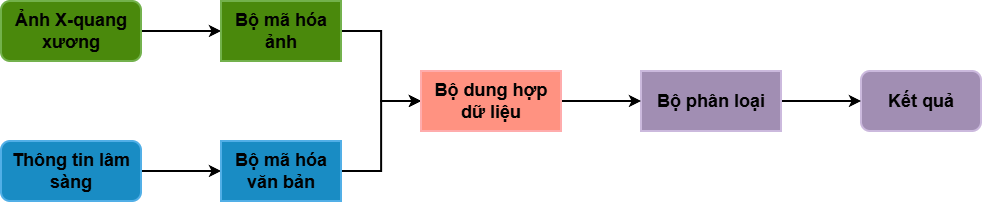
\includegraphics[width=1\linewidth]{images/Pipeline.png}
      \caption{Khung chương trình tổng quát cho một hệ thống phân loại ảnh sử dụng học sâu đa phương thức}
      \label{fig:pipeline}
  \end{figure}

Trong đó, bộ mã hóa ảnh có chức năng rút trích đặc trưng từ ảnh đầu vào, bộ mã hóa văn bản có chức năng rút trích đặc trưng từ văn bản đầu vào, bộ dung hợp dữ liệu có chức năng dung hợp hay căn chỉnh các đặc trưng được rút trích từ hai phương thức dữ liệu trên để tạo ra một biểu diễn có ý nghĩa và có đầy đủ tính chất của phương thức đầu vào, đây cũng là mô-đun quan trọng nhất đối với một mô hình học sâu đa phương thức, cuối cùng là bộ phân loại, nhận biểu diễn đặc trưng chung của các phương thức đầu vào để phân loại và đưa ra kết quả cuối cùng.

  \subsection{Mục tiêu đề tài}

Trong bối cảnh già hóa dân số và các tác nhân gây bệnh từ ô nhiễm và lối sống thiếu lành mạnh trong đời sống hiện đại, các bệnh lý về xương và chấn thương có thể ảnh hưởng trực tiếp đến đời sống và tính mạng dẫn đến việc chẩn đoán và tiên lượng để đưa ra hướng điều trị phù hợp đang trở thành gánh nặng cho các y bác sĩ, các hệ thống học sau đa phương thức tuy đã phát triển nhưng lại thiếu khả năng giải thích. Đề tài hướng đến phát triển một hệ thống phân loại ảnh X-quang có khả năng:
  \begin{itemize}
      \item Đạt được độ chính xác cao trên các bộ dữ liệu nội bộ và quốc tế.
      \item Có khả năng giải thích được kết quả.
      \item Tích hợp kết quả để trợ giúp y bác sĩ trong quá trình chẩn đoán.
  \end{itemize}

  \subsection{Phạm vi của đề tài}

Nội dung nghiên cứu của đề tài tập trung vào việc khảo sát các mô hình nền tảng và thiết kế, huấn luyện, tinh chỉnh, đánh giá kiến trúc được đề xuất trên ảnh X-quang xương và các bộ dữ liệu quốc tế để so sánh, đánh giá với các kiến trúc trước.

Đối tượng nghiên cứu xoay quanh các thành phần bên trong một mạng học sâu đa phương thức bao gồm: bộ mã hóa ảnh, bộ mã hóa văn bản, bộ dung hợp dữ liệu và bộ phân loại, tập trung vào các phương pháp dung hợp dữ liệu hình ảnh và văn bản cùng với các phương pháp tinh chỉnh tham số cho các bộ mã hóa đã được huấn luyện trước nhằm tận dụng lại các tri thức đã có và nâng cao hiệu năng trên các tác vụ đích.

Đề tài chủ yếu sử dụng các bộ dữ liệu cặp ảnh - văn bản, không có trường hợp thiếu đã được công bố và bộ dữ liệu nội bộ được thu thập và cung cấp bởi giảng viên có hợp tác với bệnh viện ở khu vực Thành phố Hồ Chí Minh, một số thông tin cơ bản về các bộ dữ liệu được thể hiện ở Bảng \ref{tab:datasets}. Nhóm sử dụng các bộ dữ liệu này nhằm đánh giá hiệu năng của kiến trúc đề xuất thông qua các độ đo phổ biến và tiến hành so sánh với các phương pháp trước đó nhằm chứng minh sự hiệu quả của phương pháp đề xuất.

  \begin{table}[htpb]
  \centering
  \resizebox{\textwidth}{!}{
  \begin{tabular}{|l|l|l|l|l|}
  \hline
  \multicolumn{1}{|c|}{\textbf{Bộ dữ liệu}} &
    \textbf{Nguồn} &
    \multicolumn{1}{c|}{\textbf{Loại dữ liệu}} &
    \multicolumn{1}{c|}{\textbf{Số lượng mẫu}} &
    \multicolumn{1}{c|}{\textbf{Số lượng lớp}} \\ \hline
  \begin{tabular}[c]{@{}l@{}}RSNA Pneumonia\\ (2018)\end{tabular} &
    \begin{tabular}[c]{@{}l@{}}Radiological  Society \\ of North America\end{tabular} &
    \begin{tabular}[c]{@{}l@{}}Ảnh X-quang ngực\\ metadata/tags\end{tabular} &
    30,000 &
    3 \\ \hline
  \begin{tabular}[c]{@{}l@{}}CheXpert\\ (2019)\end{tabular} &
    \begin{tabular}[c]{@{}l@{}}Standford ML Group -\\ Stanford Hospital\end{tabular} &
    \begin{tabular}[c]{@{}l@{}}Ảnh X-quang ngực\\ Báo cáo đọc ảnh\end{tabular} &
    224,316 &
    14 \\ \hline
  \begin{tabular}[c]{@{}l@{}}MIMIC-CXR v2\\ (2019)\end{tabular} &
    \begin{tabular}[c]{@{}l@{}}Beth Israel Deaconess \\ Medical Center\end{tabular} &
    \begin{tabular}[c]{@{}l@{}}Ảnh X-quang ngực\\ Báo cáo đọc ảnh\end{tabular} &
    227,835 &
    14 \\ \hline
  \begin{tabular}[c]{@{}l@{}}SARCOMA-CTCH\\ (2025)\end{tabular} &
    \begin{tabular}[c]{@{}l@{}}Bệnh viện Chấn Thương \\ Chỉnh Hình - TPHCM\end{tabular} &
    \begin{tabular}[c]{@{}l@{}}Ảnh X-quang xương\\ Báo cáo đọc ảnh\\ Báo cao lâm sàng\end{tabular} &
    Đang cập nhật &
    Đang cập nhật \\ \hline
  \end{tabular}
  }
  \caption{Tổng hợp các bộ dữ liệu dự kiến được sử dụng để thí nghiệm}
  \label{tab:datasets}
  \end{table}

  \subsection{Cách tiếp cận dự kiến}
Trong giai đoạn hiện nay, rất nhiều nghiên cứu về ứng dụng học sâu đa phương thức vào lĩnh vực y tế đã phát triển rất nhanh và đạt được nhiều thành tựu nổi bật. Phần này sẽ cung cấp tổng quan tình hình nghiên cứu từ đó đưa ra các nhận xét về các phương pháp hiện có làm tiền đề cho phương pháp đề xuất.

\textbf{Các mô hình xây dựng từ đầu} là các mô hình đơn giản, khởi điểm trong bài toán học sâu đa phương thức, thiết kế và huấn luyện một hệ thống mới từ đầu, điểm chung của các phương pháp này là chúng tập trung vào việc thiết kế các cơ chế để "trộn" (fusion) đặc trưng từ các bộ mã hóa (encoder) chuyên biệt ở các cấp độ khác nhau để tối ưu hóa hiệu suất cho các tác vụ cụ thể, sử dụng những bộ mã hóa hình ảnh đơn giản như CNN.

Khởi điểm vào 2020, X. Mei \cite{XMei} và đồng nghiệp đã đề xuất lấy đặc trưng được tạo ra từ các lớp cuối của mô hình CNN (véc-tơ 512 chiều) và các đặc trưng từ dữ liệu lâm sàng rồi nối lại. Véc-tơ kết hợp này được đưa vào một mạng MLP cuối cùng để đưa ra dự đoán.

Clinical-BERT \cite{yan_2022_clinicalbert} và TGANet \cite{nikhilkumartomar_2022_tganet} tìm cách học biểu diễn đa phương thức bằng cách thúc đẩy mô hình hiểu và liên kết (align) các đặc trưng giữa các vùng trong ảnh và các từ khóa trong văn bản báo cáo thông qua các nhiệm vụ tự giám sát (self-supervised objectives), cho phép mô hình học được các biểu diễn ngữ nghĩa chung. Hay LViT \cite{li_2024_lvit} đề xuất một kiến trúc hybrid CNN-Transformer "Double-U", cấu trúc CNN-Transformer kết hợp mô-đun Pixel-Level Attention Module để giữ lại các đặc trưng cục bộ của ảnh giúp mô hình giữ được khả năng trích xuất đặc trưng cục bộ mạnh mẽ của CNN, đồng thời tận dụng khả năng mô hình hóa ngữ cảnh toàn cục của Transformer.

Việc chỉ nối các đặc trưng có điểm yếu về sự khác biệt về giá trị hoặc sự ngữ nghĩa lớn giữa các phương thức dữ liệu, IRENE \cite{IRENE} đã đưa tất cả dữ liệu gốc về dạng token chung và học biểu diễn tổng thể (holistic representation) ngay từ đầu, sử dụng một mô hình Transformer duy nhất học các biểu diễn toàn diện cho cả hai phương thức. IRENE còn sử dụng cơ chế chú ý hai chiều ở cấp độ token để nắm bắt "các kết nối cục bộ".

Nghiên cứu của Dai và cộng sự \cite{TransMed21} đề xuất mô hình TransMed, giải quyết bài toán kết hợp đa phương thức bằng cách tích hợp CNN và Transformer. Bằng việc chuyển đổi đặc trưng ảnh từ CNN thành dạng chuỗi để Transformer xử lý, mô hình này tối ưu hóa việc nắm bắt các đặc điểm toàn cục của hình ảnh y khoa. Cách tiếp cận này mang lại hiệu quả cao hơn các kỹ thuật fusion thông thường nhờ khả năng biểu diễn dữ liệu đa phương thức một cách toàn diện và chính xác.

Những nghiên cứu này đã khai phá và chứng minh về tác động tích cực của các phương thức dữ liệu khác như văn bản đến kết quả của việc chẩn đoán hình ảnh, tuy nhiên độ chính xác của các phương thức này còn chưa quá cao bởi các bộ mã hóa và phương pháp dung hợp dữ liệu còn đơn giản.


  \begin{table}[htpb]
  \centering
  \resizebox{\textwidth}{!}{
  \begin{tabular}{|c|l|c|l|llll|}
  \hline
  \multirow{2}{*}{\textbf{STT}} &
    \multicolumn{1}{c|}{\multirow{2}{*}{\textbf{\begin{tabular}[c]{@{}c@{}}Tên phương \\ pháp\end{tabular}}}} &
    \multirow{2}{*}{\textbf{\begin{tabular}[c]{@{}c@{}}Chiến lược \\ tinh chỉnh\end{tabular}}} &
    \multicolumn{1}{c|}{\multirow{2}{*}{\textbf{\begin{tabular}[c]{@{}c@{}}Phương pháp \\ tinh chỉnh\end{tabular}}}} &
    \multicolumn{4}{c|}{\textbf{Kiến trúc mô hình}} \\ \cline{5-8}
    &
    \multicolumn{1}{c|}{} &
      &
    \multicolumn{1}{c|}{} &
    \multicolumn{1}{c|}{\textbf{\begin{tabular}[c]{@{}c@{}}Bộ mã hoá \\ ảnh\end{tabular}}} &
    \multicolumn{1}{c|}{\textbf{\begin{tabular}[c]{@{}c@{}}Bộ mã hoá \\ văn bản\end{tabular}}} &
    \multicolumn{1}{c|}{\textbf{\begin{tabular}[c]{@{}c@{}}Chiến lược \\ kết hợp\end{tabular}}} &
    \multicolumn{1}{c|}{\textbf{Bộ giải mã}} \\ \hline
  \textbf{1} &
    \textbf{\begin{tabular}[c]{@{}l@{}}X. Mei \cite{XMei}\end{tabular}} &
    Full Fine-Tuning &
    \begin{tabular}[c]{@{}l@{}}Pretrain với \\ Cross-Entropy loss\end{tabular} &
    \multicolumn{1}{l|}{Inception-ResNet-v2} &
    \multicolumn{1}{l|}{ResNet-18} &
    \multicolumn{1}{l|}{Decision-level} &
    N/a \\ \hline
  \textbf{2} &
    \textbf{\begin{tabular}[c]{@{}l@{}}Clinical-BERT \cite{yan_2022_clinicalbert}\end{tabular}} &
    Full Fine-Tuning &
    \begin{tabular}[c]{@{}l@{}}Cross-modal \\ Repr. Learning\end{tabular} &
    \multicolumn{1}{l|}{DenseNet121} &
    \multicolumn{1}{l|}{Uncased BERT-base} &
    \multicolumn{1}{l|}{Early fusion} &
    N/a \\ \hline
  \textbf{3} &
    \textbf{\begin{tabular}[c]{@{}l@{}}LViT \cite{li_2024_lvit}\end{tabular}} &
    Full Fine-Tuning &
    \begin{tabular}[c]{@{}l@{}}Semi-supervised \\ (Pseudo-label)\end{tabular} &
    \multicolumn{1}{l|}{\begin{tabular}[c]{@{}l@{}}Hybrid U-shape \\ (CNN + ViT)\end{tabular}} &
    \multicolumn{1}{l|}{BERT\_12\_768\_12} &
    \multicolumn{1}{l|}{Intermediate} &
    N/a \\ \hline
  \textbf{4} &
    \textbf{\begin{tabular}[c]{@{}l@{}}TGANet \cite{nikhilkumartomar_2022_tganet}\end{tabular}} &
    Train from scratch &
    \begin{tabular}[c]{@{}l@{}}Exponential Pseudo-\\ label Iteration\end{tabular} &
    \multicolumn{1}{l|}{ResNet50} &
    \multicolumn{1}{l|}{Không có} &
    \multicolumn{1}{l|}{Intermediate} &
    N/a \\ \hline
  \textbf{5} &
    \textbf{\begin{tabular}[c]{@{}l@{}}IRENE \cite{IRENE}\end{tabular}} &
    Train from scratch &
    \begin{tabular}[c]{@{}l@{}}BCE Loss \& \\ AdamW optimizer\end{tabular} &
    \multicolumn{1}{l|}{Convolution layer} &
    \multicolumn{1}{l|}{Pretrained BERT} &
    \multicolumn{1}{l|}{Simultaneous} &
    \begin{tabular}[c]{@{}l@{}}Upsampling, FEM,\\ CBAM Attention\end{tabular} \\ \hline
  \textbf{6} &
    \textbf{\begin{tabular}[c]{@{}l@{}}TransMed \cite{TransMed21}\end{tabular}} &
    Full Fine-Tuning &
    \begin{tabular}[c]{@{}l@{}} Supervised \\ (SGD, 100 epochs)\end{tabular} &
    \begin{tabular}[c]{@{}l@{}} 2D CNN \\ (ResNet18 đến 152)\end{tabular} &
    \multicolumn{1}{|l|}{N/a} &
    \multicolumn{1}{l|}{Attention fusion} &
    \begin{tabular}[c]{@{}l@{}}Lớp kết nối đầy đủ \\ (FC Layer)\end{tabular} \\ \hline
  \end{tabular}
  }
  \caption{Bảng tổng hợp chiến lược, mục tiêu và phương pháp tinh chỉnh của các mô hình kết hợp ngôn ngữ - ảnh}
  \label{tab:VLMFineTuningMethod}
\end{table}

\textbf{Mô hình ngôn ngữ trực quan y khoa (Med-VLMs)} đánh dấu một bước tiến quan trọng trong việc ứng dụng học sâu đa phương thức vào lĩnh vực y tế. Khác với các mô hình được xây dựng từ đầu (thường cố gắng dung hợp dữ liệu thô thành một khối thống nhất), Med-VLMs chú trọng vào việc đối chiếu và liên kết chặt chẽ ngữ nghĩa giữa hình ảnh và ngôn ngữ tự nhiên. Cụ thể, kiến trúc của chúng thường kế thừa các bộ mã hóa đặc trưng độc lập cho từng phương thức, điển hình như ResNet hoặc ViT cho hình ảnh và các mô hình ngôn ngữ cho văn bản. Thay vì sử dụng các mô-đun dung hợp phức tạp, Med-VLMs tối ưu hóa các hàm mất mát để căn chỉnh không gian đặc trưng của hai phương thức này khớp với nhau. Lúc này, bộ phân loại không gán nhãn theo cách truyền thống mà đóng vai trò là một cơ chế đo lường mức độ tương đồng. Nhờ biểu diễn đa phương thức mở rộng này, mô hình có khả năng thấu hiểu sâu sắc ngữ nghĩa giữa ảnh X-quang và báo cáo lâm sàng, từ đó cải thiện đáng kể hiệu năng trên nhiều tác vụ y khoa khác nhau.

Để đạt được khả năng trên, các nghiên cứu tiền huấn luyện Med-VLMs hiện nay đang phát triển chủ yếu theo ba hướng: học tương phản, học có che giấu và tích hợp tri thức y khoa (chi tiết tổng hợp được trình bày tại các Bảng \ref{tab:VLMPretrainingPrinciple}, \ref{tab:VLMPretrainingMethod}, \ref{tab:VLMPretrainingResult}).

Thứ nhất, \textbf{học tương phản (Contrastive Learning)} là chiến lược được ứng dụng rộng rãi nhất, tiêu biểu với các mô hình như ConVIRT \cite{ConVIRT}, GLoRIA \cite{GLoRIA}, MedCLIP \cite{MedCLIP} và BiomedCLIP \cite{BiomedCLIP}. Nguyên lý của chiến lược này là tối ưu hóa không gian biểu diễn bằng cách thu hẹp khoảng cách giữa các cặp đặc trưng ảnh - văn bản tương đồng, đồng thời đẩy các cặp khác biệt ra xa nhau ở mức độ cục bộ lẫn toàn cục. Phương pháp này đem lại hiệu năng ấn tượng; ví dụ, BiomedCLIP \cite{BiomedCLIP} (huấn luyện trên 15 triệu cặp dữ liệu) đạt độ chính xác phân loại 83\%, trong khi ConVIRT \cite{ConVIRT} đạt 90,3\% trên bộ dữ liệu COVIDx. Mặc dù có ưu điểm vượt trội là khả năng học biểu diễn không cần gán nhãn thủ công, học tương phản vẫn bộc lộ hạn chế về việc tiêu tốn tài nguyên tính toán lớn và rủi ro xảy ra hiện tượng âm tính giả (đẩy xa các cặp dữ liệu bị ghép nhầm dù chúng có chung đặc điểm bệnh lý).

Thứ hai, \textbf{học có che giấu (Masked Learning)} là hướng đi tập trung vào mục tiêu tái tạo dữ liệu, với các đại diện nổi bật như MRM \cite{MRM} và MedViLL \cite{MedViLL}. Bằng cách ẩn ngẫu nhiên các vùng ảnh hoặc từ ngữ trong báo cáo y khoa, kiến trúc này buộc mô hình phải dự đoán và khôi phục phần thông tin bị khuyết. Hướng tiếp cận này thể hiện ưu thế rõ rệt trong các môi trường khan hiếm dữ liệu; điển hình là MRM \cite{MRM} đạt mức 92,7\% AUC chỉ với 10\% dữ liệu từ tập RSNA. Tuy nhiên, rào cản chính của phương pháp này nằm ở việc phụ thuộc vào nguồn dữ liệu đã được ghép cặp sẵn từ trước, cộng với độ phức tạp tính toán cao của quá trình khôi phục điểm ảnh/token.

Thứ ba, \textbf{tích hợp tri thức y khoa (Knowledge Integration)} ra đời nhằm giải quyết những đặc thù phức tạp của ngôn ngữ lâm sàng. Các mô hình như MedKLIP \cite{MedKLIP}, BioViL \cite{BioViL}, BioViL-T \cite{BioViL-T} và KAD \cite{KAD} tận dụng đồ thị tri thức (như RadGraph) hoặc dữ liệu chuỗi thời gian để cung cấp tín hiệu giám sát chi tiết về cả loại và vị trí bệnh lý. Cách tiếp cận này giúp giải quyết triệt để sự mơ hồ của các từ vựng diễn tả tiến triển bệnh (ví dụ: "cải thiện", "xấu đi"). Về mặt hiệu năng, KAD \cite{KAD} đạt 0.966 AUC trên tập PadChest ở thiết lập không mẫu (zero-shot), còn BioViL-T \cite{BioViL-T} đạt độ chính xác 67,4\% trong bài toán phân loại tiến triển bệnh. Dù vậy, các phương pháp này chưa loại bỏ hoàn toàn được hiện tượng âm tính giả và rất dễ gặp sai số nếu nhãn chẩn đoán thực tế nằm ngoài cơ sở tri thức đồ thị gốc.

Dựa trên sự phân tích các ưu và nhược điểm từ những khảo sát trên, hướng tiếp cận đề xuất trong nghiên cứu này được thiết kế có chọn lọc nhằm tối ưu hóa hiệu năng và chi phí:
  \begin{itemize}
      \item \textbf{Kế thừa BiomedCLIP \cite{BiomedCLIP}:} Tận dụng sức mạnh của các bộ mã hóa đã được huấn luyện với chất lượng cao.
      \item \textbf{Không áp dụng học tương phản \& học có che giấu:} Khó khắc phục rào cản về tài nguyên tính toán lớn và giảm thiểu rủi ro gặp phải hiện tượng âm tính giả.
      \item \textbf{Tích hợp tri thức từ UMLS (tương tự MedKLIP \cite{MedKLIP}):} Sử dụng để làm giàu thêm tri thức trong các báo cáo lâm sàng.
  \end{itemize}

  \begin{table}[htpb]
  \centering
  \resizebox{\textwidth}{!}{
  \begin{tabular}{|c|l|l|l|}
  \hline
  \textbf{STT} &
    \multicolumn{1}{c|}{\textbf{\begin{tabular}[c]{@{}c@{}}Tên phương \\ pháp\end{tabular}}} &
    \multicolumn{1}{c|}{\textbf{Phân loại}} &
    \multicolumn{1}{c|}{\textbf{Nguyên lý}} \\ \hline
  \textbf{1} &
    \textbf{\begin{tabular}[c]{@{}l@{}}ConVIRT\\ (2020)\end{tabular}} &
    \begin{tabular}[c]{@{}l@{}}Học tương\\ phản\end{tabular} &
    \begin{tabular}[c]{@{}l@{}}Tối ưu bộ mã hoá ảnh và văn bản bằng cách kéo các cặp đặc trưng \\ ảnh-văn bản giống nhau lại gần nhau và đẩy các cặp đặc trưng \\ ảnh-văn bản khác nhau ra xa\end{tabular} \\ \hline
  \textbf{2} &
    \textbf{\begin{tabular}[c]{@{}l@{}}GLoRIA\\ (2021)\end{tabular}} &
    \begin{tabular}[c]{@{}l@{}}Học tương\\ phản\end{tabular} &
    \begin{tabular}[c]{@{}l@{}}Dùng hai hàm mất mát global contrastive để kéo các cặp đặc trưng \\ ảnh-văn bản, trong khi đó hàm mát mát local contrastive học cách \\ căn chỉnh chi tiết của các vùng trong ảnh và các từ trong câu\end{tabular} \\ \hline
  \textbf{3} &
    \textbf{\begin{tabular}[c]{@{}l@{}}MedCLIP\\ (2022)\end{tabular}} &
    \begin{tabular}[c]{@{}l@{}}Học tương\\ phản\end{tabular} &
    \begin{tabular}[c]{@{}l@{}}Đề xuất cơ chế tách cặp và trích xuất tri thức, và đề xuất hàm \\ mất mát Semantic Matching nhằm giải quyết vấn đề false negative\end{tabular} \\ \hline
  \textbf{4} &
    \textbf{\begin{tabular}[c]{@{}l@{}}BiomedCLIP\\ (2023)\end{tabular}} &
    \begin{tabular}[c]{@{}l@{}}Học tương\\ phản\end{tabular} &
    \begin{tabular}[c]{@{}l@{}}Có cơ chế tương tự như CLIP nhưng được tiền huấn luyện với \\ bộ dữ liệu PMC-15M\end{tabular} \\ \hline
  \textbf{5} &
    \textbf{\begin{tabular}[c]{@{}l@{}}MRM\\ (2023)\end{tabular}} &
    \begin{tabular}[c]{@{}l@{}}Học có che\\ giấu\end{tabular} &
    \begin{tabular}[c]{@{}l@{}}Ẩn ngẫu nhiên các thông tin trong văn bản và các vùng trong ảnh \\ để cho mô hình dự đoán lại ảnh và văn bản hoàn chỉnh.\end{tabular} \\ \hline
  \textbf{6} &
    \textbf{\begin{tabular}[c]{@{}l@{}}MedViLL\\ (2022)\end{tabular}} &
    \begin{tabular}[c]{@{}l@{}}Học có che\\ giấu\end{tabular} &
    \begin{tabular}[c]{@{}l@{}}Đề xuất một kiến trúc dựa trên BERT kết hợp với một mặt nạ chú ý \\ mới được đề xuất (BAR) cho phép ảnh tương tác tự do với văn bản \\ trong các tác vụ hiểu, đồng thời đảm bảo tính tự hồi quy cho các \\ token trong văn bản trong các tác vụ sinh\end{tabular} \\ \hline
  \textbf{7} &
    \textbf{\begin{tabular}[c]{@{}l@{}}BioViL\\ (2022)\end{tabular}} &
    \begin{tabular}[c]{@{}l@{}}Tích hợp\\ kiến thức\\ y khoa\end{tabular} &
    \begin{tabular}[c]{@{}l@{}}Đề xuất một bộ mã hoá văn bản CXR-BERT được tối ưu cho ảnh \\ X-quang, duy trì hàm mất mát MLM để giúp mô mình giữ lại được \\ các kiến thức văn bản trong quá trình căn chỉnh với ảnh\end{tabular} \\ \hline
  \textbf{8} &
    \textbf{\begin{tabular}[c]{@{}l@{}}BioViL-T\\ (2023)\end{tabular}} &
    \begin{tabular}[c]{@{}l@{}}Tích hợp\\ kiến thức\\ y khoa\end{tabular} &
    \begin{tabular}[c]{@{}l@{}}Sử dụng các ảnh X-quang từ trước kết hợp với ảnh hiện tại để học \\ được các đặc trưng không gian, thời gian từ đó giải thích cho các từ \\ vựng như "cải thiện" giúp giảm đi sự mơ hồ trong báo cáo\end{tabular} \\ \hline
  \textbf{9} &
    \textbf{\begin{tabular}[c]{@{}l@{}}MedKLIP\\ (2023)\end{tabular}} &
    \begin{tabular}[c]{@{}l@{}}Tích hợp\\ kiến thức\\ y khoa\end{tabular} &
    \begin{tabular}[c]{@{}l@{}}Đề xuất một mô-đun trích xuất bộ ba và cơ chế mã hoá tăng cường \\ tri thức, từ đó tạo ra biểu diển tốt hơn cho văn bản\end{tabular} \\ \hline
  \textbf{10} &
    \textbf{\begin{tabular}[c]{@{}l@{}}KAD\\ (2023)\end{tabular}} &
    \begin{tabular}[c]{@{}l@{}}Tích hợp\\ kiến thức\\ y khoa\end{tabular} &
    \begin{tabular}[c]{@{}l@{}}Tích hợp kiến thức y khoa vào quá trình tiền huấn luyện để giúp \\ mô hình học các biểu diễn có ý nghĩa hơn\end{tabular} \\ \hline
  \end{tabular}
  }
  \caption{Bảng tổng hợp nguyên lý của các phương pháp tiền huấn luyện mô hình ngôn ngữ trực quan}
  \label{tab:VLMPretrainingPrinciple}
  \end{table}

  % Please add the following required packages to your document preamble:
  % \usepackage{multirow}
  \begin{table}[htpb]
  \centering
  \resizebox{\textwidth}{!}{
  \begin{tabular}{|c|l|c|l|llll|}
  \hline
  \multirow{2}{*}{\textbf{STT}} &
    \multicolumn{1}{c|}{\multirow{2}{*}{\textbf{\begin{tabular}[c]{@{}c@{}}Tên phương \\ pháp\end{tabular}}}} &
    \multirow{2}{*}{\textbf{\begin{tabular}[c]{@{}c@{}}Chiến lược \\ tiền huấn \\ luyện\end{tabular}}} &
    \multicolumn{1}{c|}{\multirow{2}{*}{\textbf{\begin{tabular}[c]{@{}c@{}}Mục tiêu \\ tiền huấn \\ luyện\end{tabular}}}} &
    \multicolumn{4}{c|}{\textbf{Phương pháp}} \\ \cline{5-8}
    &
    \multicolumn{1}{c|}{} &
      &
    \multicolumn{1}{c|}{} &
    \multicolumn{1}{c|}{\textbf{\begin{tabular}[c]{@{}c@{}}Bộ mã hoá \\ thị giác\end{tabular}}} &
    \multicolumn{1}{c|}{\textbf{\begin{tabular}[c]{@{}c@{}}Bộ mã hoá \\ văn bản\end{tabular}}} &
    \multicolumn{1}{c|}{\textbf{\begin{tabular}[c]{@{}c@{}}Chiến lược \\ kết hợp\end{tabular}}} &
    \multicolumn{1}{c|}{\textbf{Bộ giải mã}} \\ \hline
  \textbf{1} &
    \textbf{\begin{tabular}[c]{@{}l@{}}ConVIRT\\ (2020)\end{tabular}} &
    CL &
    GCL &
    \multicolumn{1}{l|}{ResNet50} &
    \multicolumn{1}{l|}{BERT} &
    \multicolumn{1}{l|}{\begin{tabular}[c]{@{}l@{}}Contrastive \\ Alignment\end{tabular}} &
    N/a \\ \hline
  \textbf{2} &
    \textbf{\begin{tabular}[c]{@{}l@{}}GLoRIA\\ (2021)\end{tabular}} &
    CL &
    LCL, GCL &
    \multicolumn{1}{l|}{ResNet50} &
    \multicolumn{1}{l|}{BioClinicalBERT} &
    \multicolumn{1}{l|}{\begin{tabular}[c]{@{}l@{}}Global-Local \\ Contrastive \\ Alignment\end{tabular}} &
    N/a \\ \hline
  \textbf{3} &
    \textbf{\begin{tabular}[c]{@{}l@{}}MedCLIP\\ (2022)\end{tabular}} &
    CL &
    GCL &
    \multicolumn{1}{l|}{\begin{tabular}[c]{@{}l@{}}Swin Transformer, \\ ResNet50\end{tabular}} &
    \multicolumn{1}{l|}{BioClinicalBERT} &
    \multicolumn{1}{l|}{\begin{tabular}[c]{@{}l@{}}Knowledge-enhanced \\ Alignment\end{tabular}} &
    N/a \\ \hline
  \textbf{4} &
    \textbf{\begin{tabular}[c]{@{}l@{}}BiomedCLIP\\ (2023)\end{tabular}} &
    CL &
    GCL &
    \multicolumn{1}{l|}{ViT-Base} &
    \multicolumn{1}{l|}{PubMedBERT} &
    \multicolumn{1}{l|}{\begin{tabular}[c]{@{}l@{}}Contrastive \\ Alignment\end{tabular}} &
    N/a \\ \hline
  \textbf{5} &
    \textbf{\begin{tabular}[c]{@{}l@{}}MRM\\ (2023)\end{tabular}} &
    MP &
    MIM, MLM &
    \multicolumn{1}{l|}{\begin{tabular}[c]{@{}l@{}}Kiến trúc \\ giống ViT\end{tabular}} &
    \multicolumn{1}{l|}{WordPiece} &
    \multicolumn{1}{l|}{\begin{tabular}[c]{@{}l@{}}Global Context \\ Injection\end{tabular}} &
    \begin{tabular}[c]{@{}l@{}}Văn bản: Transformer;\\ Hình ảnh: Fully Connected\end{tabular} \\ \hline
  \textbf{6} &
    \textbf{\begin{tabular}[c]{@{}l@{}}MedViLL\\ (2022)\end{tabular}} &
    HA &
    MLM, ITM &
    \multicolumn{1}{l|}{ResNet50} &
    \multicolumn{1}{l|}{BERT} &
    \multicolumn{1}{l|}{\begin{tabular}[c]{@{}l@{}}Cross-modal \\ Self-Attention\end{tabular}} &
    Multi-Layer Perceptron \\ \hline
  \textbf{7} &
    \textbf{\begin{tabular}[c]{@{}l@{}}BioViL\\ (2022)\end{tabular}} &
    HA &
    CL, MLM &
    \multicolumn{1}{l|}{ResNet50} &
    \multicolumn{1}{l|}{CXR-BERT} &
    \multicolumn{1}{l|}{\begin{tabular}[c]{@{}l@{}}Global-Local \\ Contrastive \\ Alignment\end{tabular}} &
    N/A \\ \hline
  \textbf{8} &
    \textbf{\begin{tabular}[c]{@{}l@{}}BioViL-T\\ (2023)\end{tabular}} &
    HA &
    CL, MLM &
    \multicolumn{1}{l|}{ResNet50} &
    \multicolumn{1}{l|}{CXR-BERT} &
    \multicolumn{1}{l|}{\begin{tabular}[c]{@{}l@{}}Global-Local \\ Contrastive \\ Alignment\end{tabular}} &
    N/A \\ \hline
  \textbf{9} &
    \textbf{\begin{tabular}[c]{@{}l@{}}MedKLIP\\ (2023)\end{tabular}} &
    CL &
    LCL &
    \multicolumn{1}{l|}{ResNet50} &
    \multicolumn{1}{l|}{ClinicalBERT} &
    \multicolumn{1}{l|}{\begin{tabular}[c]{@{}l@{}}Knowledge-enhanced \\ Alignment\end{tabular}} &
    \begin{tabular}[c]{@{}l@{}}Constrative head, \\ Cross-Entroy head\end{tabular} \\ \hline
  \textbf{10} &
    \textbf{\begin{tabular}[c]{@{}l@{}}KAD\\ (2023)\end{tabular}} &
    HA &
    \begin{tabular}[c]{@{}l@{}}CL, Disease \\ Diagnosis \\ Prediction\end{tabular} &
    \multicolumn{1}{l|}{\begin{tabular}[c]{@{}l@{}}ResNet50, \\ ViT-Base\end{tabular}} &
    \multicolumn{1}{l|}{PubMedBERT} &
    \multicolumn{1}{l|}{\begin{tabular}[c]{@{}l@{}}Contrastive \\ Alignment\end{tabular}} &
    Disease Query Network \\ \hline
  \end{tabular}
  }
  \caption{Bảng tổng hợp chiến lược, mục tiêu và phương pháp tiền huấn luyện của các mô hình ngôn ngữ trực quan. Trong đó, CL (Contrastive Learning): Học tương phản; GCL (Global Contrastive Learning): Học tương phản toàn cục; LCL (Local Contrastive Learning): Học tương phản cục bộ; MIM (Masked Image Modeling): Mô hình hóa hình ảnh có che giấu; MLM (Masked Language Modeling): Mô hình hóa ngôn ngữ có che giấu; ITM (Image-Text Matching): Ghép nối ảnh - văn bản;}
  \label{tab:VLMPretrainingMethod}
  \end{table}

  % Please add the following required packages to your document preamble:
  % \usepackage{multirow}
  \begin{table}[htpb]
  \centering
  \resizebox{\textwidth}{!}{
  \begin{tabular}{|c|l|l|llll|}
  \hline
  \multirow{2}{*}{\textbf{STT}} &
    \multicolumn{1}{c|}{\multirow{2}{*}{\textbf{\begin{tabular}[c]{@{}c@{}}Tên phương \\ pháp\end{tabular}}}} &
    \multicolumn{1}{c|}{\multirow{2}{*}{\textbf{\begin{tabular}[c]{@{}c@{}}Bộ dữ liệu\\ tiền huấn luyện\end{tabular}}}} &
    \multicolumn{4}{c|}{\textbf{Hiệu năng}} \\ \cline{4-7}
    &
    \multicolumn{1}{c|}{} &
    \multicolumn{1}{c|}{} &
    \multicolumn{1}{c|}{\textbf{Tác vụ}} &
    \multicolumn{1}{c|}{\textbf{\begin{tabular}[c]{@{}c@{}}Bộ dữ liệu\\ đánh giá\end{tabular}}} &
    \multicolumn{1}{c|}{\textbf{Độ đo}} &
    \multicolumn{1}{c|}{\textbf{Kết quả}} \\ \hline
  \textbf{1} &
    \textbf{\begin{tabular}[c]{@{}l@{}}ConVIRT\\ (2020)\end{tabular}} &
    \begin{tabular}[c]{@{}l@{}}MIMIC-CXR, \\ Private Bone image\end{tabular} &
    \multicolumn{1}{l|}{\begin{tabular}[c]{@{}l@{}}- Phân loại ảnh\\ - Phân loại ít mẫu\end{tabular}} &
    \multicolumn{1}{l|}{\begin{tabular}[c]{@{}l@{}}RSNA Pneumonia, \\ CheXpert, COVIDx, \\ MURA\end{tabular}} &
    \multicolumn{1}{l|}{\begin{tabular}[c]{@{}l@{}}AUC,\\ Accuracy\end{tabular}} &
    \begin{tabular}[c]{@{}l@{}}- Phân loại ít mẫu: RSNA (1\%): 88.8\% AUC, \\ (10\%): 91.5\% AUC; CheXpert (1\%): 87.0\% AUC, \\ (10\%): 88.1\% AUC; MURA (1\%): 81.3\% AUC, \\ (10\%): 86.5\% AUC\\ - Phân loại ảnh: RSNA: 92.7\% AUC, \\ CheXpert: 88.1\% AUC, MURA: 89.0\% AUC; \\ COVIDx 90.3\% ACC\end{tabular} \\ \hline
  \textbf{2} &
    \textbf{\begin{tabular}[c]{@{}l@{}}GLoRIA\\ (2021)\end{tabular}} &
    CheXpert &
    \multicolumn{1}{l|}{\begin{tabular}[c]{@{}l@{}}- Phân loại ảnh\\ - Phân loại ít mẫu\\ - Phân loại không mẫu\end{tabular}} &
    \multicolumn{1}{l|}{\begin{tabular}[c]{@{}l@{}}CheXpert, RSNA \\ Pneumonia\end{tabular}} &
    \multicolumn{1}{l|}{AUROC} &
    \begin{tabular}[c]{@{}l@{}}- Phân loại không mẫu: CheXpert 5x200: 0.61 ACC, \\ 0.67 F1; RSNA: 0.70 ACC, 0.58 F1; \\ - Phân loại ít mẫu: CheXpert (1\%): 86.6 AUC, \\ (10\%): 87.8 AUC, RSNA (1\%): 86.1 AUC, \\ (10\%) 88.0 AUC\\ - Phân loại ảnh: CheXpert: 88.1 AUC, \\ RSNA: 88.6 AUC\end{tabular} \\ \hline
  \textbf{3} &
    \textbf{\begin{tabular}[c]{@{}l@{}}MedCLIP\\ (2022)\end{tabular}} &
    \begin{tabular}[c]{@{}l@{}}MIMIC-CXR, \\ CheXpert\end{tabular} &
    \multicolumn{1}{l|}{\begin{tabular}[c]{@{}l@{}}- Phân loại ảnh\\ - Phân loại không mẫu\end{tabular}} &
    \multicolumn{1}{l|}{\begin{tabular}[c]{@{}l@{}}MIMIC-5x200, \\ COVID, RSNA \\ Pneumonia\end{tabular}} &
    \multicolumn{1}{l|}{\begin{tabular}[c]{@{}l@{}}Mean \\ Accuracy\end{tabular}} &
    \begin{tabular}[c]{@{}l@{}}- Phân loại không mẫu: \\ CheXpert-5x200: 0.5942 ACC; \\ MIMIC-5x200: 0.5430 ACC; COVID: 0.8472 ACC; \\ RSNA: 0.7682 ACC\\ - Phân loại ảnh: CheXpert-5x200: 0.5960 ACC; \\ MIMIC-5x200: 0.5650 ACC; COVID: 0.7890 ACC; \\ RSNA: 0.8075 ACC\end{tabular} \\ \hline
  \textbf{4} &
    \textbf{\begin{tabular}[c]{@{}l@{}}BiomedCLIP\\ (2023)\end{tabular}} &
    PMC-15M &
    \multicolumn{1}{l|}{\begin{tabular}[c]{@{}l@{}}- Phân loại ảnh\\ - Phân loại ít mẫu\\ - Phân loại không mẫu\end{tabular}} &
    \multicolumn{1}{l|}{\begin{tabular}[c]{@{}l@{}}PCam, LC25000 \\ (Lung, Colon), \\ TCGA-TIL, RSNA \\ Pneumonia\end{tabular}} &
    \multicolumn{1}{l|}{\begin{tabular}[c]{@{}l@{}}AUC,\\ Accuracy\end{tabular}} &
    \begin{tabular}[c]{@{}l@{}}- Phân loại không mẫu: PCam: 73.41\% ACC; \\ LC25000 Lung 65.23\% ACC; LC25000 Colon 92.98\%; \\ RSNA 78.95\%; TCGA-TIL: 67.04\%\\ - Phân loại ít mẫu: PCam (1\%): 82\% ACC, (10\%): 83\%; \\ RSNA (1\%): 77\% ACC, (10\%): 82\% ACC\\ - Phân loại ảnh: PCam: 83\% ACC, RSNA: 83\% ACC\end{tabular} \\ \hline
  \textbf{5} &
    \textbf{\begin{tabular}[c]{@{}l@{}}MRM\\ (2023)\end{tabular}} &
    MIMIC-CXR &
    \multicolumn{1}{l|}{\begin{tabular}[c]{@{}l@{}}- Phân loại ảnh\\ - Phân loại ít mẫu\end{tabular}} &
    \multicolumn{1}{l|}{\begin{tabular}[c]{@{}l@{}}CheXpert, NIH \\ ChestX-ray, RSNA \\ Pneumonia, COVID-19 \\ Image Data Collection\end{tabular}} &
    \multicolumn{1}{l|}{\begin{tabular}[c]{@{}l@{}}AUC, \\ Accuracy\end{tabular}} &
    \begin{tabular}[c]{@{}l@{}}- Phân loại ít mẫu: CheXpert (1\%): 88.5 AUC, \\ (10\%): 88.5 AUC; RSNA (1\%): 91.3 AUC, \\ (10\%): 92.7 AUC; NIH ChestX-ray (1\%): 79.4 AUC, \\ (10\%): 84.0 AUC\\ - Phân loại ảnh: CheXpert: 88.7 AUC, RSNA 93.3, \\ NIH ChestX-ray: 85.9, COVID-19: 85.8\end{tabular} \\ \hline
  \textbf{6} &
    \textbf{\begin{tabular}[c]{@{}l@{}}MedViLL\\ (2022)\end{tabular}} &
    MIMIC-CXR &
    \multicolumn{1}{l|}{- Phân loại chẩn đoán} &
    \multicolumn{1}{l|}{MIMIC-CXR, Open-I} &
    \multicolumn{1}{l|}{\begin{tabular}[c]{@{}l@{}}Micro-averaged \\ AUROC,\\ Micro-averaged \\ F1 score\end{tabular}} &
    \begin{tabular}[c]{@{}l@{}}- Phân loại ảnh: MIMIC-CXR: 0.980 avg AUROC, \\ 0.839 F1; Open-I: 0.892 avg AUROC, 0.407 F1\end{tabular} \\ \hline
  \textbf{7} &
    \textbf{\begin{tabular}[c]{@{}l@{}}BioViL\\ (2022)\end{tabular}} &
    MIMIC-CXR &
    \multicolumn{1}{l|}{\begin{tabular}[c]{@{}l@{}}- Phân loại ảnh\\ - Phân loại ít mẫu\\ - Phân loại không mẫu\end{tabular}} &
    \multicolumn{1}{l|}{RSNA Pneumonia} &
    \multicolumn{1}{l|}{\begin{tabular}[c]{@{}l@{}}Accuracy, \\ F1-score, \\ AUROC, \\ Sensitivity\\ Specificity.\end{tabular}} &
    \begin{tabular}[c]{@{}l@{}}- Phân loại không mẫu: RSNA: 0.732 ACC, 0.831 AUC; \\ ChestX-ray14: 0.6912 AUC\\ - Phân loại ít mẫu: RSNA (1\%): 0.805 ACC, 0.881 AUC; \\ (10\%): 0.812 ACC, 0.884 AUC\\ - Phân loại ảnh: RSNA: 0.822 ACC, 0.891 AUC\end{tabular} \\ \hline
  \textbf{8} &
    \textbf{\begin{tabular}[c]{@{}l@{}}BioViL-T\\ (2023)\end{tabular}} &
    MIMIC-CXR &
    \multicolumn{1}{l|}{\begin{tabular}[c]{@{}l@{}}- Phân loại ảnh\\ - Phân loại ít mẫu\\ - Phân loại không mẫu\\ - Phân loại ảnh tiến triển\end{tabular}} &
    \multicolumn{1}{l|}{\begin{tabular}[c]{@{}l@{}}MS-CXR-T, RSNA \\ Penumonia, Chest \\ ImaGenome\end{tabular}} &
    \multicolumn{1}{l|}{\begin{tabular}[c]{@{}l@{}}Macro-Accuracy, \\ Accuracy, F1, \\ AUROC.\end{tabular}} &
    \begin{tabular}[c]{@{}l@{}}- Phân loại Tiến triển: MS-CXR-T: 67.4\% Acc\\ - Phân loại không mẫu: RSNA: 0.805 ACC, 0.871 AUC\\ - Phân loại ít mẫu: RSNA (1\%): 0.814 ACC, 0.890 AUC\end{tabular} \\ \hline
  \textbf{9} &
    \textbf{\begin{tabular}[c]{@{}l@{}}MedKLIP\\ (2023)\end{tabular}} &
    MIMIC-CXR &
    \multicolumn{1}{l|}{\begin{tabular}[c]{@{}l@{}}- Phân loại ảnh\\ - Phân loại không mẫu\end{tabular}} &
    \multicolumn{1}{l|}{\begin{tabular}[c]{@{}l@{}}ChestX-ray14, RSNA \\ Pneumonia, SIIM-ACR \\ Pneumothorax, COVIDx \\ CXR-2, COVID Rural, \\ Edema Severity\end{tabular}} &
    \multicolumn{1}{l|}{\begin{tabular}[c]{@{}l@{}}AUC, \\ F1-score, \\ Accuracy.\end{tabular}} &
    \begin{tabular}[c]{@{}l@{}}- Phân loại không mẫu: RSNA: 0.8694 AUC, 0.6342 F1; \\ SIIM-ACR: 0.8924 AUC, 0.6833 F1; \\ ChestX-ray14: 0.7676 AUC, 0.2525 F1; \\ COVID-19: 0.7396 AUC, 0.7670 F1\\ - Phân loại ít mẫu: ChestX-ray14 (1\%): 0.7721 AUC, \\ (10\%): 0.7894; RSNA (1\%): 0.8731 AUC, \\ (10\%): 0.8799 AUC\\ - Phân loại mẫu: ChestX-ray14: 0.8323 AUC, \\ RSNA 0.8931\end{tabular} \\ \hline
  \textbf{10} &
    \textbf{\begin{tabular}[c]{@{}l@{}}KAD\\ (2023)\end{tabular}} &
    MIMIC-CXR &
    \multicolumn{1}{l|}{\begin{tabular}[c]{@{}l@{}}- Phân loại ảnh\\ - Phân loại ít mẫu\\ - Phân loại không mẫu\end{tabular}} &
    \multicolumn{1}{l|}{\begin{tabular}[c]{@{}l@{}}PadChest, NIH \\ ChestXray14, CheXpert, \\ ChestX-Det\end{tabular}} &
    \multicolumn{1}{l|}{\begin{tabular}[c]{@{}l@{}}AUC, \\ F1-Score, \\ MCC\end{tabular}} &
    \begin{tabular}[c]{@{}l@{}}- Phân loại không mẫu: PadChest: 0.966 AUC; \\ CheXpert: 0.905 AUC, 0.647 F1, 0.589 MCC\\ - Phân loại ít mẫu: ChestXray-14 (1\%): 0.78 AUC, \\ 0.31 F1; (10\%): 0.80 AUC, 0.33 F1\\ - Phân loại ảnh: ChestXray-14: 0.82 AUC, 0.34 F1\end{tabular} \\ \hline
  \end{tabular}
  }
  \caption{Bảng tổng hợp kết quả của các phương pháp tiền huấn luyện mô hình ngôn ngữ trực quan}
  \label{tab:VLMPretrainingResult}
  \end{table}

Mặc dù các phương pháp tiền huấn luyện Med-VLMs giúp xây dựng nền tảng tri thức đa phương thức khổng lồ, việc áp dụng trực tiếp vào lâm sàng lại vấp phải rào cản lớn về chi phí tính toán và sự khan hiếm dữ liệu y tế ghép cặp. Để giải quyết vấn đề này, các nghiên cứu thường chuyển hướng sang tinh chỉnh mô hình. Tuy nhiên, nếu tinh chỉnh toàn phần trên một tập dữ liệu nhỏ, sự chênh lệch phân phối sẽ dễ dẫn đến hiện tượng chuyển giao tiêu cực hoặc "quên thảm khốc", làm đánh mất tri thức gốc. Do đó, giới nghiên cứu đang tập trung vào các chiến lược tinh chỉnh hiệu quả tham số (PEFT) nhằm đảm bảo tính linh hoạt, tiết kiệm tài nguyên và giữ vững khả năng tổng quát hóa. Dựa trên cơ chế can thiệp, các nghiên cứu gần đây được chia thành ba hướng tiếp cận chính:

\pagebreak

\textbf{Tinh chỉnh sử dụng câu nhắc (Prompt Tuning):} Hướng này chèn thêm các tham số có thể học được vào không gian đầu vào của mô hình. Các phương pháp như CITE \cite{CITE}, FPT \cite{FPT} hay PLIP \cite{PLIP} khai thác đặc trưng thị giác kết hợp với tri thức lâm sàng, cho thấy hiệu quả vượt trội ngay cả khi thiếu hụt dữ liệu (ví dụ: PLIP đạt 0.896 AUC chỉ với 5\% dữ liệu PanNuke). Nhằm giải quyết khó khăn khi thiết kế thủ công, MedPrompt \cite{MedPrompt} và UniDCP \cite{UniDCP} tự động sinh câu nhắc động dựa trên ngữ cảnh ảnh để xử lý đa tác vụ. Gần đây hơn, việc tích hợp Mô hình ngôn ngữ Lớn (LLM) qua ViP \cite{ViP}, CILMP \cite{CLIMP} và BiomedCoOp \cite{BiomedCoOp} giúp tạo sinh các câu nhắc ngữ nghĩa sâu sắc, đồng bộ hóa qua cơ chế chú ý chéo và căn chỉnh tương phản, mang lại hiệu năng cao trong các kịch bản ít mẫu hoặc không mẫu.

\textbf{Tinh chỉnh bộ điều hợp (Adapter Tuning):} Thay vì can thiệp ở đầu vào, phương pháp này chèn các mô-đun mạng nơ-ron siêu nhẹ giữa các lớp của kiến trúc gốc. Điển hình, CLIPath \cite{CLIPath} sử dụng kết nối thặng dư để giảm khoảng cách miền trên dữ liệu nhỏ; FTB \cite{FTB} đặt mô-đun dung hợp giữa bộ mã hóa ảnh và văn bản để chắt lọc thông tin đa phương thức. Ở hướng bán giám sát, mô hình MedUnA \cite{MedUnA} dùng LLM tạo nhãn giả và tinh chỉnh không giám sát bộ điều hợp trên ảnh chưa gán nhãn, giúp mô hình thích ứng tốt mà không thay đổi trọng số.

\textbf{Tinh chỉnh chọn lọc (Selective Tuning):} Hướng đi này tối ưu hóa kiến trúc bằng cách chỉ cập nhật một lượng nhỏ các trọng số quyết định hiệu năng. TransMed \cite{TransMed} kết hợp LLM để chuyển đổi nhãn bệnh thành mô tả chi tiết, trong khi SH-PEFT \cite{SH-PEFT} chỉ tìm và cập nhật các trọng số quan trọng nhất trên bộ mã hóa thị giác nhằm khai thác tính thưa thớt của mạng. Tương tự, LCBB \cite{LCBB} áp dụng kỹ thuật LoRA để tinh chỉnh tham số hiệu quả cho Med-VLMs, giúp bám sát hiệu năng của tinh chỉnh toàn phần (đạt 93.1\% AUROC trên tập RSNA với 10\% dữ liệu gán nhãn) nhưng giảm thiểu tối đa chi phí tính toán.

  % Please add the following required packages to your document preamble:
  % \usepackage{multirow}
  \begin{table}[htpb]
  \centering
  \resizebox{\textwidth}{!}{
  \begin{tabular}{|c|l|l|l|llll|}
  \hline
  \multirow{2}{*}{\textbf{STT}} &
    \multicolumn{1}{c|}{\multirow{2}{*}{\textbf{\begin{tabular}[c]{@{}c@{}}Tên phương \\ pháp\end{tabular}}}} &
    \multicolumn{1}{c|}{\multirow{2}{*}{\textbf{\begin{tabular}[c]{@{}c@{}}Chiến lược \\ tinh chỉnh\end{tabular}}}} &
    \multicolumn{1}{c|}{\multirow{2}{*}{\textbf{\begin{tabular}[c]{@{}c@{}}Phương pháp \\ tinh chỉnh\end{tabular}}}} &
    \multicolumn{4}{c|}{\textbf{Phương pháp}} \\ \cline{5-8}
    &
    \multicolumn{1}{c|}{} &
    \multicolumn{1}{c|}{} &
    \multicolumn{1}{c|}{} &
    \multicolumn{1}{c|}{\textbf{\begin{tabular}[c]{@{}c@{}}Bộ mã hoá \\ thị giác\end{tabular}}} &
    \multicolumn{1}{c|}{\textbf{\begin{tabular}[c]{@{}c@{}}Bộ mã hoá \\ văn bản\end{tabular}}} &
    \multicolumn{1}{c|}{\textbf{\begin{tabular}[c]{@{}c@{}}Chiến lược \\ kết hợp\end{tabular}}} &
    \multicolumn{1}{c|}{\textbf{Bộ giải mã}} \\ \hline
  \textbf{1} &
    \textbf{\begin{tabular}[c]{@{}l@{}}CITE\\ (2023)\end{tabular}} &
    \begin{tabular}[c]{@{}l@{}}Parameter-efficient \\ fine tuning\end{tabular} &
    \begin{tabular}[c]{@{}l@{}}Visual prompt \\ tuning\end{tabular} &
    \multicolumn{1}{l|}{\begin{tabular}[c]{@{}l@{}}CLIP ViT-Base, \\ ImageNet-21k ViT-Base, \\ INTERN ViT-Base\end{tabular}} &
    \multicolumn{1}{l|}{\begin{tabular}[c]{@{}l@{}}BioLinkBERT-large, \\ BioBERT-large , \\ Kế thừa CLIP\end{tabular}} &
    \multicolumn{1}{l|}{\begin{tabular}[c]{@{}l@{}}Contrastive \\ Alignment\end{tabular}} &
    N/a \\ \hline
  \textbf{2} &
    \textbf{\begin{tabular}[c]{@{}l@{}}UniDCP\\ (2023)\end{tabular}} &
    \begin{tabular}[c]{@{}l@{}}Parameter-efficient \\ fine tuning\end{tabular} &
    \begin{tabular}[c]{@{}l@{}}Visual-Textual \\ prompt tuning\end{tabular} &
    \multicolumn{1}{l|}{CLIP ViT} &
    \multicolumn{1}{l|}{RoBERTa} &
    \multicolumn{1}{l|}{\begin{tabular}[c]{@{}l@{}}Cross Attention, \\ Contrastive \\ Alignment\end{tabular}} &
    N/a \\ \hline
  \textbf{3} &
    \textbf{\begin{tabular}[c]{@{}l@{}}ViP\\ (2024)\end{tabular}} &
    \begin{tabular}[c]{@{}l@{}}Parameter-efficient \\ fine tuning\end{tabular} &
    \begin{tabular}[c]{@{}l@{}}Textual prompt \\ tuning\end{tabular} &
    \multicolumn{1}{l|}{ViT-Base} &
    \multicolumn{1}{l|}{Kế thừa CLIP} &
    \multicolumn{1}{l|}{\begin{tabular}[c]{@{}l@{}}Cross Attention, \\ Contrastive \\ Alignment\end{tabular}} &
    N/a \\ \hline
  \textbf{4} &
    \textbf{\begin{tabular}[c]{@{}l@{}}PLIP\\ (2024)\end{tabular}} &
    \begin{tabular}[c]{@{}l@{}}Parameter-efficient \\ fine tuning\end{tabular} &
    \begin{tabular}[c]{@{}l@{}}Visual prompt \\ tuning, Efficient \\ Selective tuning\end{tabular} &
    \multicolumn{1}{l|}{ViT-Base} &
    \multicolumn{1}{l|}{Kế thừa CLIP} &
    \multicolumn{1}{l|}{Concatnate} &
    N/a \\ \hline
  \textbf{5} &
    \textbf{\begin{tabular}[c]{@{}l@{}}FPT\\ (2024)\end{tabular}} &
    \begin{tabular}[c]{@{}l@{}}Parameter-efficient \\ fine tuning\end{tabular} &
    \begin{tabular}[c]{@{}l@{}}Visual prompt \\ tuning\end{tabular} &
    \multicolumn{1}{l|}{ViT-Base} &
    \multicolumn{1}{l|}{N/a} &
    \multicolumn{1}{l|}{Cross Attention} &
    N/a \\ \hline
  \textbf{6} &
    \textbf{\begin{tabular}[c]{@{}l@{}}MedPrompt\\ (2024)\end{tabular}} &
    \begin{tabular}[c]{@{}l@{}}Parameter-efficient \\ fine tuning\end{tabular} &
    \begin{tabular}[c]{@{}l@{}}Textual prompt \\ tuning\end{tabular} &
    \multicolumn{1}{l|}{\begin{tabular}[c]{@{}l@{}}Swin Transformer, \\ ResNet50\end{tabular}} &
    \multicolumn{1}{l|}{Kế thừa CLIP} &
    \multicolumn{1}{l|}{\begin{tabular}[c]{@{}l@{}}Contrastive \\ Alignment\end{tabular}} &
    N/a \\ \hline
  \textbf{7} &
    \textbf{\begin{tabular}[c]{@{}l@{}}CILMP\\ (2025)\end{tabular}} &
    \begin{tabular}[c]{@{}l@{}}Parameter-efficient \\ fine tuning\end{tabular} &
    \begin{tabular}[c]{@{}l@{}}Visual-Textual \\ prompt tuning\end{tabular} &
    \multicolumn{1}{l|}{ViT-Base} &
    \multicolumn{1}{l|}{Kế thừa CLIP} &
    \multicolumn{1}{l|}{\begin{tabular}[c]{@{}l@{}}Hadamard Product, \\ Concatnate\end{tabular}} &
    N/a \\ \hline
  \textbf{8} &
    \textbf{\begin{tabular}[c]{@{}l@{}}BiomedCoOp\\ (2025)\end{tabular}} &
    \begin{tabular}[c]{@{}l@{}}Parameter-efficient \\ fine tuning\end{tabular} &
    \begin{tabular}[c]{@{}l@{}}Visual-Textual \\ prompt tuning\end{tabular} &
    \multicolumn{1}{l|}{Kế thừa BiomedCLIP} &
    \multicolumn{1}{l|}{Kế thừa BiomedCLIP} &
    \multicolumn{1}{l|}{\begin{tabular}[c]{@{}l@{}}Contrastive \\ Alignment\end{tabular}} &
    N/a \\ \hline
  \textbf{9} &
    \textbf{\begin{tabular}[c]{@{}l@{}}CLIPath\\ (2023)\end{tabular}} &
    \begin{tabular}[c]{@{}l@{}}Parameter-efficient \\ fine tuning\end{tabular} &
    \begin{tabular}[c]{@{}l@{}}Adapter \\ tuning\end{tabular} &
    \multicolumn{1}{l|}{ResNet50} &
    \multicolumn{1}{l|}{Kế thừa CLIP} &
    \multicolumn{1}{l|}{\begin{tabular}[c]{@{}l@{}}Contrastive \\ Alignment\end{tabular}} &
    N/a \\ \hline
  \textbf{10} &
    \textbf{\begin{tabular}[c]{@{}l@{}}FTB\\ (2024)\end{tabular}} &
    \begin{tabular}[c]{@{}l@{}}Parameter-efficient \\ fine tuning\end{tabular} &
    \begin{tabular}[c]{@{}l@{}}Adapter \\ tuning\end{tabular} &
    \multicolumn{1}{l|}{\begin{tabular}[c]{@{}l@{}}ResNet autoencoder, \\ DINOv2-small, \\ DINOv2-base\end{tabular}} &
    \multicolumn{1}{l|}{\begin{tabular}[c]{@{}l@{}}BERT, \\ BioBERT, \\ ClinicalBERT, \\ CXR-BERT, \\ PubMedBERT\end{tabular}} &
    \multicolumn{1}{l|}{Cross Attention} &
    N/a \\ \hline
  \textbf{11} &
    \textbf{\begin{tabular}[c]{@{}l@{}}MedUnA\\ (2024)\end{tabular}} &
    \begin{tabular}[c]{@{}l@{}}Parameter-efficient \\ fine tuning\end{tabular} &
    \begin{tabular}[c]{@{}l@{}}Adapter \\ tuning\end{tabular} &
    \multicolumn{1}{l|}{\begin{tabular}[c]{@{}l@{}}ViT-Base, \\ MedCLIP-Swin\end{tabular}} &
    \multicolumn{1}{l|}{\begin{tabular}[c]{@{}l@{}}Kế thừa CLIP, \\ MedCLIP\end{tabular}} &
    \multicolumn{1}{l|}{No Fusion} &
    N/a \\ \hline
  \textbf{12} &
    \textbf{\begin{tabular}[c]{@{}l@{}}TransMed\\ (2023)\end{tabular}} &
    \begin{tabular}[c]{@{}l@{}}Parameter-efficient \\ fine tuning\end{tabular} &
    \begin{tabular}[c]{@{}l@{}}Direct Selective \\ tuning\end{tabular} &
    \multicolumn{1}{l|}{\begin{tabular}[c]{@{}l@{}}Swin Transformer, \\ ViT-Base\end{tabular}} &
    \multicolumn{1}{l|}{BERT, LLM/GPT-4} &
    \multicolumn{1}{l|}{\begin{tabular}[c]{@{}l@{}}Contrastive \\ Alignment\end{tabular}} &
    N/a \\ \hline
  \textbf{13} &
    \textbf{\begin{tabular}[c]{@{}l@{}}SH-PEFT\\ (2024)\end{tabular}} &
    \begin{tabular}[c]{@{}l@{}}Parameter-efficient \\ fine tuning\end{tabular} &
    \begin{tabular}[c]{@{}l@{}}Direct Selective \\ tuning\end{tabular} &
    \multicolumn{1}{l|}{ViT-Base} &
    \multicolumn{1}{l|}{Kế thừa CLIP} &
    \multicolumn{1}{l|}{No Fusion} &
    N/a \\ \hline
  \textbf{14} &
    \textbf{\begin{tabular}[c]{@{}l@{}}LCBB\\ (2024)\end{tabular}} &
    \begin{tabular}[c]{@{}l@{}}Parameter-efficient \\ fine tuning\end{tabular} &
    \begin{tabular}[c]{@{}l@{}}Efficient Selective \\ tuning\end{tabular} &
    \multicolumn{1}{l|}{\begin{tabular}[c]{@{}l@{}}Kế thừa MAE, \\ MRM\end{tabular}} &
    \multicolumn{1}{l|}{\begin{tabular}[c]{@{}l@{}}Kế thừa MAE, \\ MRM\end{tabular}} &
    \multicolumn{1}{l|}{\begin{tabular}[c]{@{}l@{}}Kế thừa MAE, \\ MRM\end{tabular}} &
    N/a \\ \hline
  \end{tabular}
  }
  \caption{Bảng tổng hợp chiến lược, mục tiêu và phương pháp học chuyển giao của các mô hình ngôn ngữ trực quan}
  \label{tab:VLMTransferlearningMethod}
  \end{table}

Tóm lại, các phương pháp tinh chỉnh hiệu quả tham số (PEFT) thể hiện ưu điểm vượt trội trong việc tiết kiệm tài nguyên tính toán, ngăn chặn hiện tượng quên tri thức và giúp mô hình thích ứng tốt ngay cả khi đối mặt với các bộ dữ liệu y tế khan hiếm. Tuy nhiên, hướng tiếp cận này vẫn tồn tại một số hạn chế nhất định. Hiệu năng cuối cùng của hệ thống phụ thuộc rất lớn vào chất lượng của mô hình tiền huấn luyện gốc. Đồng thời, quá trình thiết kế câu nhắc mang đậm tính chuyên môn hay xác định vị trí tối ưu để chèn bộ điều hợp thường phức tạp và đòi hỏi nhiều thử nghiệm. Ngoài ra, việc bổ sung các thành phần này ít nhiều làm tăng tính "hộp đen" của mô hình, gây ra những thách thức về tính minh bạch khi cần giải thích các quyết định dự đoán cho bác sĩ trên thực tế lâm sàng.

\textbf{Các mô hình ngôn ngữ lớn y khoa đa phương thức}

Trong thời gian gần đây, với sự phát triển của các mô hình ngôn ngữ lớn được huấn luyện trên những tập dữ liệu rất lớn phục vụ cho rất nhiều tác vụ khác nhau, các mô hình này đang thể hiện sự ảnh hưởng và đa dụng trong lĩnh vực y tế với độ chính xác rất tốt khi chỉ học ít mẫu hoặc không mẫu.

Med-Flamingo \cite{moor_2023_medflamingo} là mô hình đầu tiên có khả năng học ít mẫu chuyên dụng cho y tế, thông qua hội thoại tự nhiên để hỗ trợ chẩn đoán. Theo sau đó, LLaVA-Med \cite{li_2023_llavamed} là mô hình chuyển đổi khả năng thực hiện theo chỉ dẫn (instruction-following) từ miền tổng quát sang lĩnh vực y sinh bằng cách sử dụng dữ liệu cặp ảnh-văn bản quy mô lớn với 600.000 cặp, với dữ liệu hội thoại tạo ra từ chú thích ảnh y khoa được tạo ra bằng cách sử dụng GPT-4. Phương pháp này đã đề xuất quy trình huấn luyện 2 bước: (1) Căn chỉnh khái niệm; (2) Tinh chỉnh chỉ dẫn đầy đủ; 2 bước này tương ứng với giai đoạn học và suy luận. Kết quả thể hiện khả năng suy luận vượt trội trên dữ liệu chưa từng thấy.

Med-Palm M \cite{MED-PALM-M} là mô hình của Google, đánh dấu bước tiến từ các mô hình đơn nhiệm sang đa nhiệm quy mô lớn, có khả năng xử lý đa nhiệm và đa phương thức bằng một bộ tham số duy nhất, thay vì sử dụng các mô hình chuyên biệt cho từng tác vụ. Gần đây hơn, SkinGPT-4 \cite{SkinGPT-4} là hệ thống chẩn đoán da liễu tương tác đầu tiên sử dụng LLM quy mô lớn với độ chính xác cao, đã kết hợp khả năng hiểu hình ảnh y tế chuyên sâu với khả năng suy luận và giao tiếp của các mô hình ngôn ngữ lớn (LLM), tạo ra một hệ thống chẩn đoán da liễu có thể tương tác, giải thích lý do và đưa ra lời khuyên hữu ích cho người dùng.

Dù đưa đến các phương pháp có độ chính xác cao đến rất cao trong nhiều tác vụ cùng việc hỗ trợ trong việc giao tiếp với mô hình, kích cỡ và chi phí huấn luyện (Med-Flamingo có đến 9 tỷ thông số) để vận hành các mô hình ngôn ngữ lớn đa phương thức là một vấn đề lớn, đi kèm với vấn đề ảo giác có thể gặp phải khi đối mặt mới dữ liệu mới hoặc những câu hỏi phức tạp. Ngoài ra nếu yêu cầu một độ chính xác cao - một yêu cầu quan trọng trong lĩnh vực y tế trong một tác vụ cụ thể thì đây không phải một cách tiếp cận tốt cho bài toán này.

  \begin{table}[htpb]
  \centering
  \scriptsize
  \setlength{\tabcolsep}{3pt}

  \begin{adjustbox}{max width=\textwidth}
  \begin{tabular}{|c|l|c|l|llll|}
  \hline
  \multirow{2}{*}{\textbf{STT}} &
    \multicolumn{1}{c|}{\multirow{2}{*}{\textbf{\begin{tabular}[c]{@{}c@{}}Tên phương \\ pháp\end{tabular}}}} &
    \multirow{2}{*}{\textbf{\begin{tabular}[c]{@{}c@{}}Chiến lược \\ tinh chỉnh\end{tabular}}} &
    \multicolumn{1}{c|}{\multirow{2}{*}{\textbf{\begin{tabular}[c]{@{}c@{}}Phương pháp \\ tinh chỉnh\end{tabular}}}} &
    \multicolumn{4}{c|}{\textbf{Cấu trúc phương pháp}} \\ \cline{5-8}
    &
    \multicolumn{1}{c|}{} &
      &
    \multicolumn{1}{c|}{} &
    \multicolumn{1}{c|}{\textbf{\begin{tabular}[c]{@{}c@{}}Bộ mã hoá \\ ảnh\end{tabular}}} &
    \multicolumn{1}{c|}{\textbf{\begin{tabular}[c]{@{}c@{}}Bộ mã hoá \\ văn bản\end{tabular}}} &
    \multicolumn{1}{c|}{\textbf{\begin{tabular}[c]{@{}c@{}}Chiến lược \\ kết hợp\end{tabular}}} &
    \multicolumn{1}{c|}{\textbf{Bộ giải mã}} \\ \hline

  \textbf{1} &
    \textbf{Med-Flamingo \cite{moor_2023_medflamingo}} &
    PEFT &
    \begin{tabular}[c]{@{}l@{}}Parameter-efficient \\ + Domain adaptation\end{tabular} &
    \multicolumn{1}{l|}{Frozen CLIP ViT} &
    \multicolumn{1}{l|}{LLaMA-7B} &
    \multicolumn{1}{l|}{\begin{tabular}[c]{@{}l@{}}Intermediate \\ fusion\end{tabular}} &
    LLaMA Decoder \\ \hline

  \textbf{2} &
    \textbf{LLaVA-Med \cite{li_2023_llavamed}} &
    Full FT &
    \begin{tabular}[c]{@{}l@{}}Visual Instruction \\ Tuning (GPT-4 data)\end{tabular} &
    \multicolumn{1}{l|}{CLIP ViT-L/14} &
    \multicolumn{1}{l|}{LLaMA} &
    \multicolumn{1}{l|}{\begin{tabular}[c]{@{}l@{}}Projection \\ Matrix\end{tabular}} &
    LLM (Vicuna) \\ \hline

  \textbf{3} &
    \textbf{Med-PaLM M \cite{MED-PALM-M}} &
    Full FT &
    Instruction Fine-tuning &
    \multicolumn{1}{l|}{ViT (4B - 22B)} &
    \multicolumn{1}{l|}{PaLM} &
    \multicolumn{1}{l|}{\begin{tabular}[c]{@{}l@{}}Multimodal \\ embedding\end{tabular}} &
    PaLM \\ \hline

  \textbf{4} &
    \textbf{SkinGPT-4 \cite{SkinGPT-4}} &
    PEFT &
    LoRA &
    \multicolumn{1}{l|}{Vision Transformer} &
    \multicolumn{1}{l|}{GPT-4} &
    \multicolumn{1}{l|}{\begin{tabular}[c]{@{}l@{}}Linear \\ alignment\end{tabular}} &
    LLaMA-2-13B \\ \hline
  \end{tabular}
  \end{adjustbox}
  \caption{Tổng hợp chiến lược và cấu trúc các mô hình ngôn ngữ lớn đa phương thức}
  \label{tab:MedVLM_Comparison}
\end{table}

\textbf{Phương pháp đề xuất:} Dựa trên các nghiên cứu liên quan, nhóm đề xuất xây dựng một hệ thống học sâu đa phương thức nhằm khai thác đồng thời thông tin từ ảnh X-quang và dữ liệu lâm sàng văn bản. Đặc biệt, hệ thống được thiết kế theo hướng tích hợp tri thức y khoa nhằm nâng cao khả năng giải thích của mô hình được minh họa ở Hình \ref{fig:proposed}. Cụ thể, kiến trúc bao gồm các thành phần chính như sau:
  \begin{itemize}
      \item \textbf{Bộ mã hóa ảnh:} Kế thừa lại mô hình ViT-Base của phương pháp BiomedCLIP \cite{BiomedCLIP}
      \item \textbf{Bộ mã hóa văn bản:} Kế thừa lại mô hình PubMedBERT của phương pháp BiomedCLIP \cite{BiomedCLIP}
      \item \textbf{Bộ dung hợp dữ liệu:} Nhóm hướng đến sử dụng cơ chế \textbf{\textit{Knowledge-guided Cross-Attention}} - Các khái niệm y học được trích xuất và liên kết từ văn bản lâm sàng thông qua sẽ được sử dụng để tạo thiên lệch (bias) trong quá trình tính toán cross attention. Cơ chế này giúp điều hướng mô hình tập trung vào các vùng ảnh có liên quan đến bệnh lý, thay vì các vùng nền không liên quan. Nhờ đó, mô hình không chỉ cải thiện hiệu năng mà còn cung cấp khả năng giải thích thông qua việc truy vết mối liên hệ giữa khái niệm y khoa và vùng ảnh được chú ý.
      \item \textbf{Bộ phân loại:} Sử dụng một mạng phân loại (Multi-Layer Perceptron) để dự đoán nhãn bệnh lý.
  \end{itemize}
Đồng thời, các trọng số attention và thông tin từ tri thức y khoa được khai thác để trực quan hóa và giải thích kết quả dự đoán.

  \begin{figure}[H]
\centering
      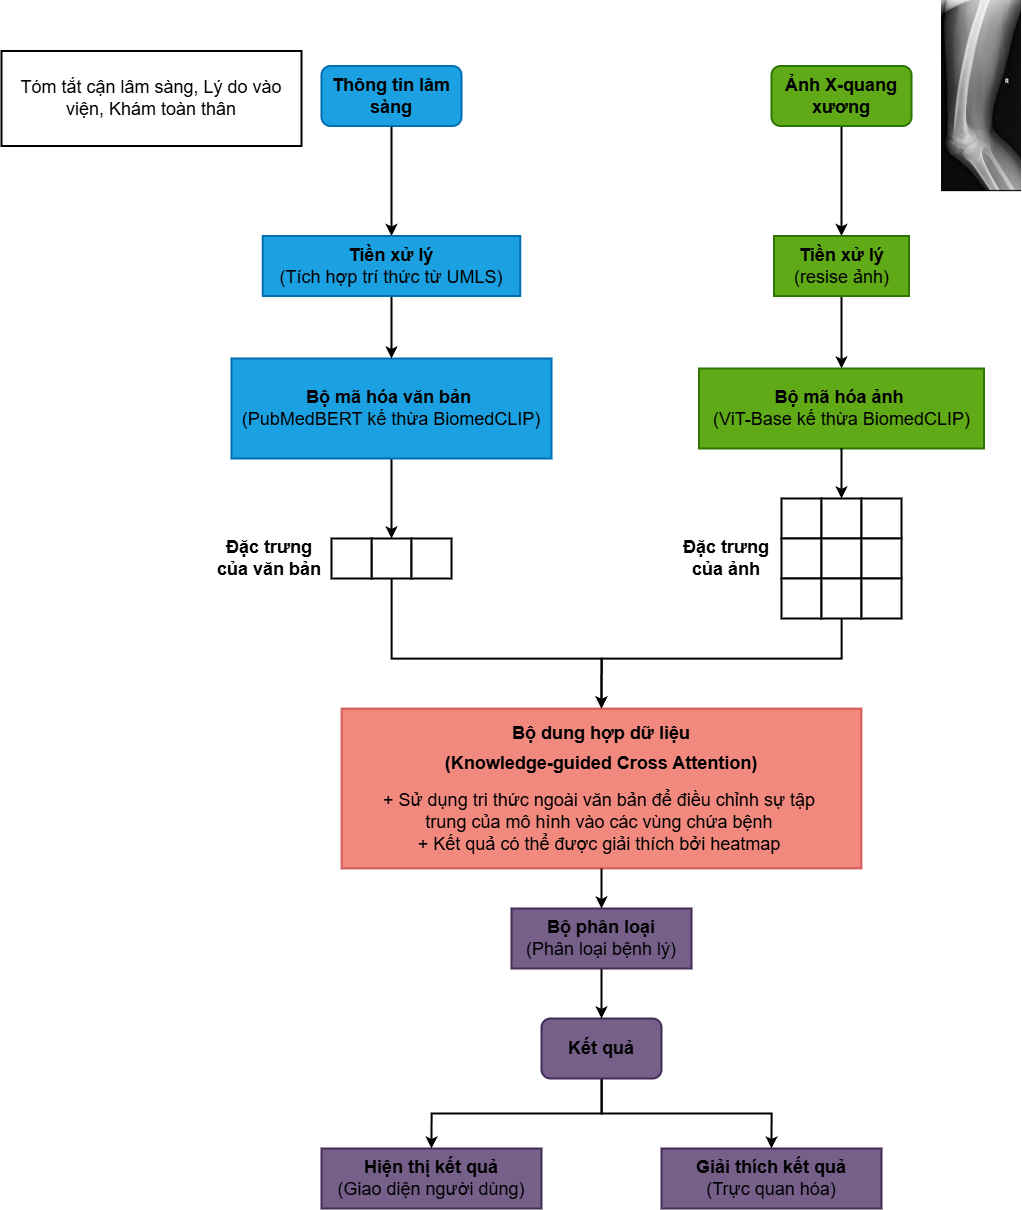
\includegraphics[width=1\linewidth]{images/thesis_pipeline.png}
      \caption{Kiến trúc tổng thể của hệ thống đề xuất}
      \label{fig:proposed}
  \end{figure}

  \subsection{Kết quả dự kiến của đề tài}

  \begin{itemize}
      \item \textbf{Số liệu định lượng:} Độ chính xác, điểm F1, AUC-ROC đạt kết quả cạnh tranh trên các bộ dữ liệu đã nêu.

      \item \textbf{Sản phẩm đầu ra:}
      \begin{itemize}
          \item Hệ thống demo phân loại ảnh X-quang xương với khả năng nhận ảnh và văn bản và trả ra các lớp thuộc bộ dữ liệu Sarcoma-CTCH.

          \item Giao diện đơn giản để hiển thị kết quả phân loại.

          \item Cho phép trực quan hóa sau khi hiện kết quả phân loại.
      \end{itemize}

      \item \textbf{Báo cáo khoa học:} hoàn thiện phương pháp và hệ thống để hướng tới công bố trên các hội nghị và tạp chí uy tín trong lĩnh vực Trí tuệ nhân tạo và Y sinh, như MICCAI, CVPR hoặc các tạp chí được công nhận.

      \item \textbf{Hướng phát triển:}
      \begin{itemize}
          \item Mở rộng ra cho các bệnh lý khác.
          \item Cải thiện độ chính xác và hiệu suất của hệ thống.
      \end{itemize}
  \end{itemize}

\pagebreak

  \subsection{Kế hoạch thực hiện}
  % Please add the following required packages to your document preamble:
  % \usepackage{multirow}
  \begin{table}[htpb]
  \centering
  \resizebox{\textwidth}{!}{
  \begin{tabular}{|c|l|ll|}
  \hline
  \textbf{Mục tiêu} &
    \multicolumn{1}{c|}{\textbf{Thời gian}} &
    \multicolumn{1}{l|}{\textbf{Phân công}} &
    \multicolumn{1}{c|}{\textbf{Nội dung}} \\ \hline
  \multirow{16}{*}{\textbf{\begin{tabular}[c]{@{}c@{}}Khoá luận \\ tốt nghiệp\end{tabular}}} &
    \multirow{4}{*}{\textbf{01 tháng}} &
    \multicolumn{2}{c|}{\textbf{Giai đoạn 1}} \\ \cline{3-4}
    &                                     & \multicolumn{1}{l|}{\textbf{Bá Thành}} & Khảo sát tổng quan về bài toán phân loại ảnh X-quang về xương \\ \cline{3-4}
    &                                     & \multicolumn{1}{l|}{\textbf{Gia Kiệt}} & Khảo sát các mô hình tiền huấn luyện trên dữ liệu y khoa      \\ \cline{3-4}
    &
      &
    \multicolumn{1}{l|}{\textbf{Bá Thành}} &
    \begin{tabular}[c]{@{}l@{}}Khảo sát các phương pháp học chuyển giao và các mô hình \\ liên quan\end{tabular} \\ \cline{2-4}
    & \multirow{4}{*}{\textbf{02 tháng}}  & \multicolumn{2}{c|}{\textbf{Giai đoạn 2}}                                                              \\ \cline{3-4}
    &
      &
    \multicolumn{1}{l|}{\textbf{Cả nhóm}} &
    \begin{tabular}[c]{@{}l@{}}Phát triển mô hình học sâu đa phương thức áp dụng \\ phương pháp học chuyển giao\end{tabular} \\ \cline{3-4}
    &                                     & \multicolumn{1}{l|}{\textbf{Gia Kiệt}} & Cài đặt môi trường, thu thập các bộ dữ liệu liên quan         \\ \cline{3-4}
    &                                     & \multicolumn{1}{l|}{\textbf{Bá Thành}} & Thực hiện thí nghiệm trên mô hình đề xuất                     \\ \cline{2-4}
    & \multirow{3}{*}{\textbf{02 tháng}}  & \multicolumn{2}{c|}{\textbf{Giai đoạn 3}}                                                              \\ \cline{3-4}
    &                                     & \multicolumn{1}{l|}{\textbf{Bá Thành}} & Phân tích so sánh kết quả thực nghiệm.                        \\ \cline{3-4}
    &                                     & \multicolumn{1}{l|}{\textbf{Gia Kiệt}} & Xây dựng nguyên mẫu cho hệ thống phân loại                    \\ \cline{2-4}
    & \multirow{2}{*}{\textbf{0.5 tháng}} & \multicolumn{2}{c|}{\textbf{Giai đoạn 4}}                                                              \\ \cline{3-4}
    &
      &
    \multicolumn{1}{l|}{\textbf{Cả nhóm}} &
    \begin{tabular}[c]{@{}l@{}}Viết 01 bài báo khoa học cho hội nghị - tạp chí chuyên ngành \\ trong nước hoặc ngoài nước\end{tabular} \\ \cline{2-4}
    & \multirow{3}{*}{\textbf{0.5 tháng}} & \multicolumn{2}{c|}{\textbf{Giai đoạn 5}}                                                              \\ \cline{3-4}
    &                                     & \multicolumn{1}{l|}{\textbf{Bá Thành}} & Viết báo cáo khoá luận tốt nghiệp.                            \\ \cline{3-4}
    &                                     & \multicolumn{1}{l|}{\textbf{Gia Kiệt}} & Thiết kế slide cho lễ bảo vệ đề tài tốt nghiệp                \\ \hline
  \end{tabular}
  }
  \caption{Kế hoạch bố trí thời gian nghiên cứu}
  \label{tab:plan}
  \end{table}
\pagebreak \nocite{*} \printbibliography[heading=subbibliography, title={Tài liệu tham khảo}]

\vspace{1.5cm} \noindent \hfill
  \begin{minipage}[t]{0.4\textwidth}
\centering
      \fontsize{12}{16}\textbf{XÁC NHẬN\\CỦA NGƯỜI HƯỚNG DẪN}\\
\fontsize{12}{16}\textit{(Ký và ghi rõ họ tên)}
  \end{minipage}%
\hfill
  \begin{minipage}[t]{0.6\textwidth}
\centering
      \fontsize{12}{16}\textit{TP. Hồ Chí Minh, ngày 05 tháng 04 năm 2026}\\
      \fontsize{12}{16}\textbf{NHÓM SINH VIÊN THỰC HIỆN}\\
\fontsize{12}{16}\textit{(Ký và ghi rõ họ tên)}
  \end{minipage}%
\hfill\null \normalsize
\endgroup






